\section{Process Scheduling}

	\defn{I/O Bound}{a process which spends most of its time doing I/O instead of computations}

	\defn{CPU Bound}{a process which spends most of its time doing computations}

	\defn{Multiprogramming}{when theres a process running at all times}

	\defn{Time Sharing}{switch among several different processes quickly enough so as to give the impression of parallel execution}

	\defn{Long-Term Scheduler}{is responsible for maintaining a healthy balance between IO and CPU bound processes in memory}

	\defn{Medium-Term Scheduler}{swaps processes from active to passive and vice-versa}

	\defn{Short-Term Scheduler}{selects which process to execute next}

	\par{Even with multiple cores, if there are more processes then cores then some processes will need to wait before they're able to run. Hence, there is the need for some sort of scheduling of processes. The main goal of the scheduler is to maximize CPU utilization at all times, in order to achieve this there exist several types of schedulers and several queues need to be maintained in order to keep track of each process state.}

	\begin{figure}[H]
		\begin{center}
		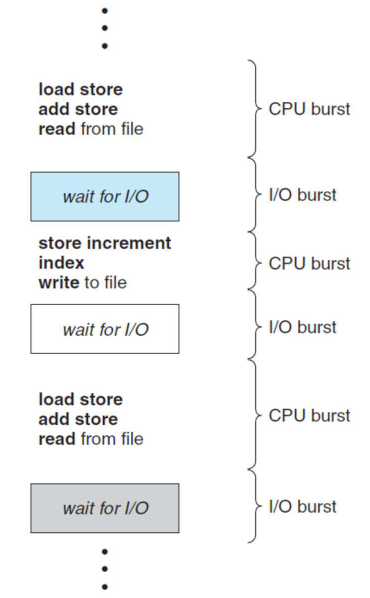
\includegraphics[width=0.75\textwidth , height=0.25\textwidth]{processLife}
		\end{center}
	\end{figure}

	\par{The \ita{job scheduler} concerns itself with loading programs into memory, the \ita{medium-term} one performs possibly necessary swaps between active/holding states and the \ita{CPU scheduler} decides which process to execute next. These 3 schedulers can move processes among the various queues : all processes exist first in the \ita{job queue}, once they are in RAM and ready to execute they are put into the \ita{ready queue}, if the process is waiting for a particular device then it is put into that device's queue.} 

	\begin{figure}[H]
		\begin{center}
		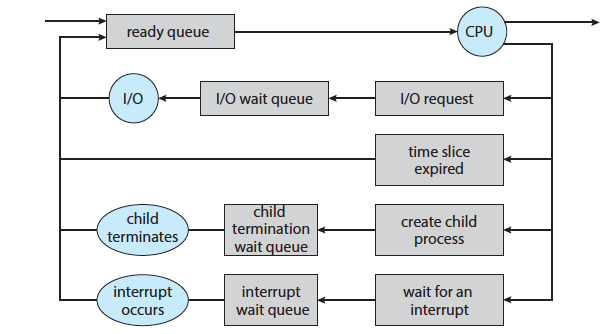
\includegraphics[width=\textwidth]{sched}
		\end{center}
	\end{figure}

	\subsection{CPU Scheduler}

		\defn{Non-Preemptive Scheduling}{let the process run its course without interruption}

		\defn{Preemptive Scheduling}{the process decides when the process should yield the CPU}

		\par{As discussed a process may switch several times between one of the queues and the CPU, though CPU bound processes will spend more time executing it is unlikely that the scheduler will grant long chunks of uninterrupted time to these processes. Instead, processes in the core are constantly interrupted and switched.}

		\rem{It is common for the CPU scheduler to execute much more frequently than once every 100ms}

		\par{When to decide when to schedule a process to run in the core may take place at any of 4 stages of a life of a process:}

			\begin{itemize}
				\item[] Running $\to$ Waiting (e.g I/O request)
				\item[] Running $\to$ Ready (e.g interrupt)
				\item[] Waiting $\to$ Ready (e.g I/O terminates)
				\item[] Termination 
			\end{itemize}

	\subsection{Dispatcher}

		\defn{Dispatch Latency}{is the time it takes the dispatcher to switch processes}

		\par{It is the job of the dispatcher to give control of the CPU to the process selected by the scheduler. In order to do this the scheduler must be able to \ita{switch context}, \ita{switch to user mode} and \ita{jump back to the proper instruction in the user program to resume execution}}

		\rem{Given that the dispatcher is called every time a process is swapped and the time it takes to do so is pure overhead, it is important that it be as fast possible. }

	\subsection{Scheduling Criteria}

		\par{The best algorithm for a particular process may not be the best for another set of processes. It is important that one is aware of this fact when choosing an algorithm. In order to compare them, the following criteria can be used:}

			\begin{itemize}
				\item[]CPU Utilization : maximize , in practice somewhere between $40\%-90\%$
				\item[]Throughput : maximize , for any given time unit, one aims to complete as many processes as possible 
				\item[]Waiting Time : minimize , waiting time is wasted time
				\item[]Turnaround Time : minimize , the aim is faster total completion times 
				\item[]Response Time : minimize , in an interactive system this criteria can be better than turnaround time, we measure when the first response is issued
			\end{itemize}

			\example{ Find below the application of each algorithm for the following processes:

			$$\begin{array}{|l|l|l|}\hline \begin{array}{l}\text { Process ID } \\ \text { (PID) }\end{array} & \begin{array}{l}\text { Arrival } \\ \text { Time }\end{array} & \begin{array}{l}\text { CPU Burst } \\ \text { Time }\end{array} \\ \hline \text { P1 } & 0 & 6 \\ \hline \text { P2 } & 4 & 14 \\ \hline \text { P3 } & 5 & 10 \\ \hline\end{array}$$
			}

	\subsection{FIFO}

		\par{The \ita{First-In First-Out} algorithm, is a non-preemptive algorithm which executes the processes in order of arrival. It is very simple to implement but can lead to large waiting times}

	\begin{figure}[H]
		\begin{center}
		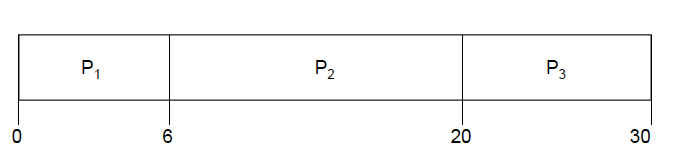
\includegraphics[width=\textwidth]{FIFO}
		\end{center}
		\begin{center}
		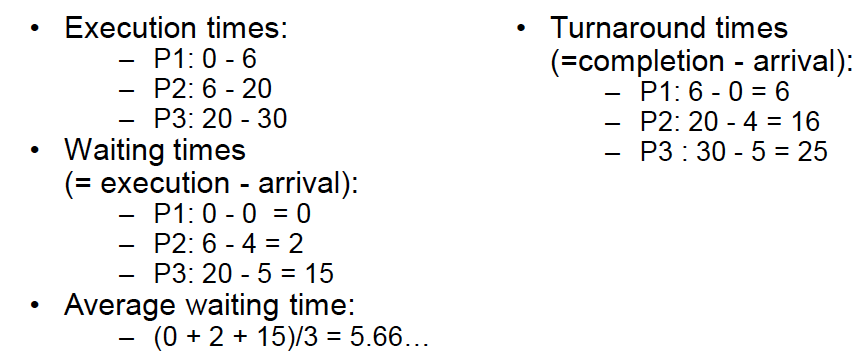
\includegraphics[width=\textwidth]{FIFOc}
		\end{center}
	\end{figure}

	\subsection{SJF}

		\par{The \ita{Shortest Job First} algorithm chooses the processes with the lowest CPU burst time to be executed first, if the processes have the same CPU burst time then it falls back to FIFO. This is also simple to implement, but an obvious problem is that processes with large CPU burst times may take much more to implement}

		\begin{figure}[H]
		\begin{center}
		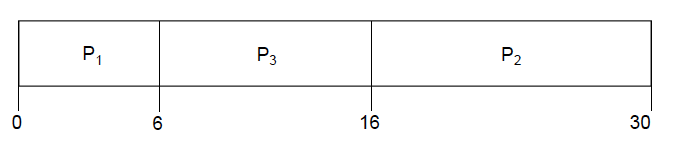
\includegraphics[width=\textwidth]{SJF}
		\end{center}
		\begin{center}
		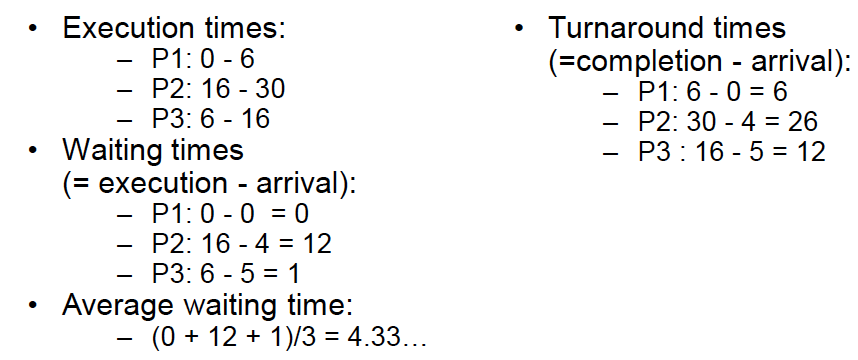
\includegraphics[width=\textwidth]{SJFc}
		\end{center}
	\end{figure}

	\subsection{SRTF}

		\par{The \ita{Shortest Remaining Time First} is a preemptive version of SJF, i.e. it looks at the list of processes in the ready queue with each new arrival and compares the total remaining completion times, if the total time of a waiting process is lower than the one currently in execution then it will interrupt execution and swap them. }

		\begin{figure}[H]
		\begin{center}
		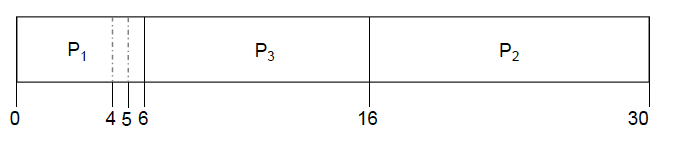
\includegraphics[width=\textwidth]{SRTF}
		\end{center}
		\begin{center}
		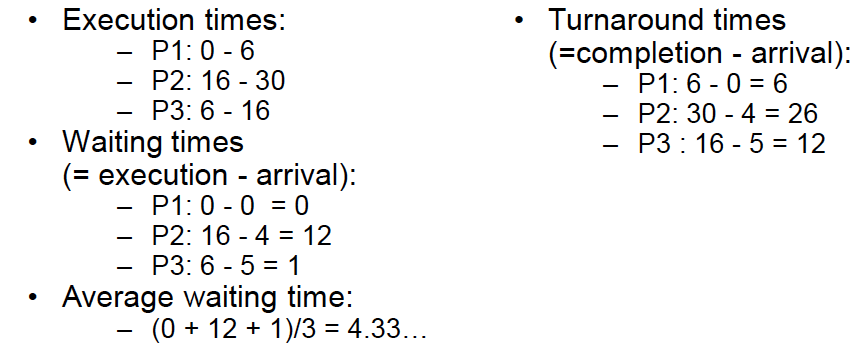
\includegraphics[width=\textwidth]{SRTFc}
		\end{center}
	\end{figure}

	\subsection{NPP}

		\par{The \ita{Non-Preemptive Priority Scheduling} adds processes to a queue according to their priority values; if processes share the same priority level, then it reverts back to FIFO. It is also fairly simple to implement, but similarly to SJF it might lead to \ita{starvation}, i.e processes with low priority may take ages or never run}

		\begin{figure}[H]
		\begin{center}
		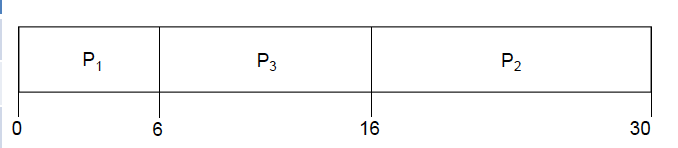
\includegraphics[width=\textwidth]{NPP}
		\end{center}
		\begin{center}
		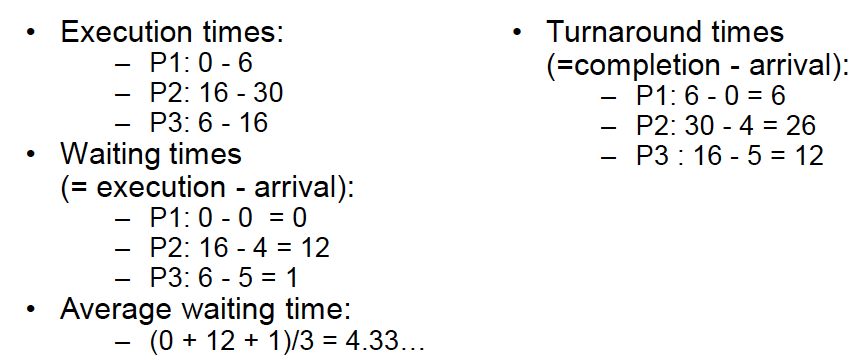
\includegraphics[width=\textwidth]{NPPc}
		\end{center}
	\end{figure}

	\subsection{RR}

		\par{The \ita{Round-Robin Scheduling} is the preemptive version of FIFO, where processes are executed according to time of arrival but only for a certain time period - \ita{quantum}. If the process finished early then the dispatcher moves down the queue, if the opposite happens the process is added to the back of the queue.}

		\begin{figure}[H]
		\begin{center}
		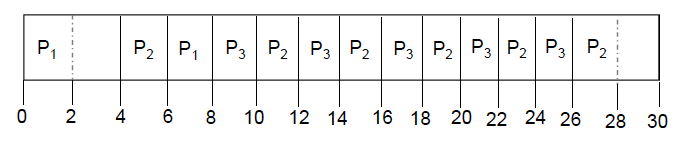
\includegraphics[width=\textwidth]{RR}
		\end{center}
		\begin{center}
		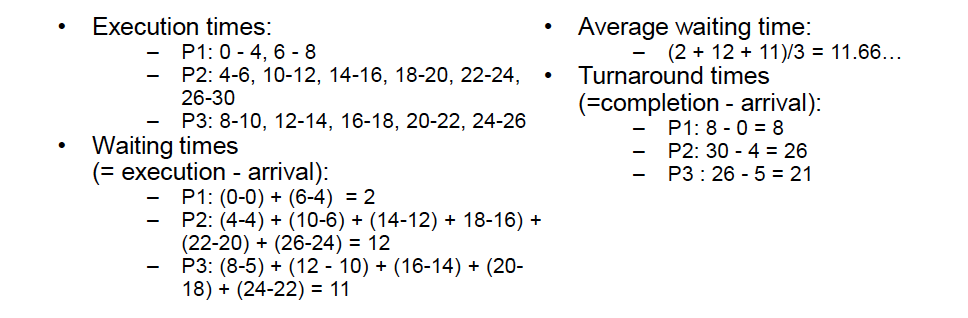
\includegraphics[width=\textwidth]{RRc}
		\end{center}
	\end{figure}

	\subsection{MQ}

		\par{The \ita{Multilevel Queue Scheduling} separates processes according to their priority values into separate queues. This has the advantage of reducing the time taken to search through all processes since it needs only to look at the highest-priority queue. It is then often combined with RR to decide which process within a queue should be executed next }


























